\section{Aprendizaje automático}

\noindent
En la literatura más tradicional de IA, se acostumbra motivar y guiar la teoría por medio de\
las capacidades y limitaciones de un \textbf{agente} (racional). Esto es una abstracción de un ente real,\
capaz de percibir información de su ambiente, procesarla y tomar decisiones. El agente será\
equipado del conocimiento necesario para decidir la mejor opción según lo que exista en su entorno.\par
La arquitectura interna del agente se compone de una máquina finita de \emph{estados} (con sus variantes),\
cuyas transiciones están determinadas por \emph{reglas de interpretación}. Cada vez que un agente\
cambia de estado, se produce una \emph{acción}. La naturaleza de esta estructura nos lleva a reducir\
muchos de los problemas de la IA en búsquedas, en las cuales el agente puede o no saber \emph{a priori}\
el conjunto de posibles resultados que puede encontrar.\par
Computacionalmente hablando, el espacio de búsqueda de varios problemas interesantes en IA se vuelve\
bastante intratable, por lo que no es posible simplemente codificar todos los posibles escenarios\
dentro de la \emph{base de conocimientos} de un agente. El camino hacia la solución a este problema\
comienza con dos observaciones:
\begin{itemize}
\item un agente puede (y debe) ser capaz de manejar la incertidumbre de su entorno dependiendo\
  de la verosimilitud de un evento;
\item el cerebro humano pasa mucho tiempo adquiriendo conocimiento a través de experiencias\
  que previamente \emph{aprendió}, por ende, no es descabellado enseñar a un agente a que\
  automáticamente se genere una descripción de su entorno.
\end{itemize}

\begin{figure}[H]
  \centering
  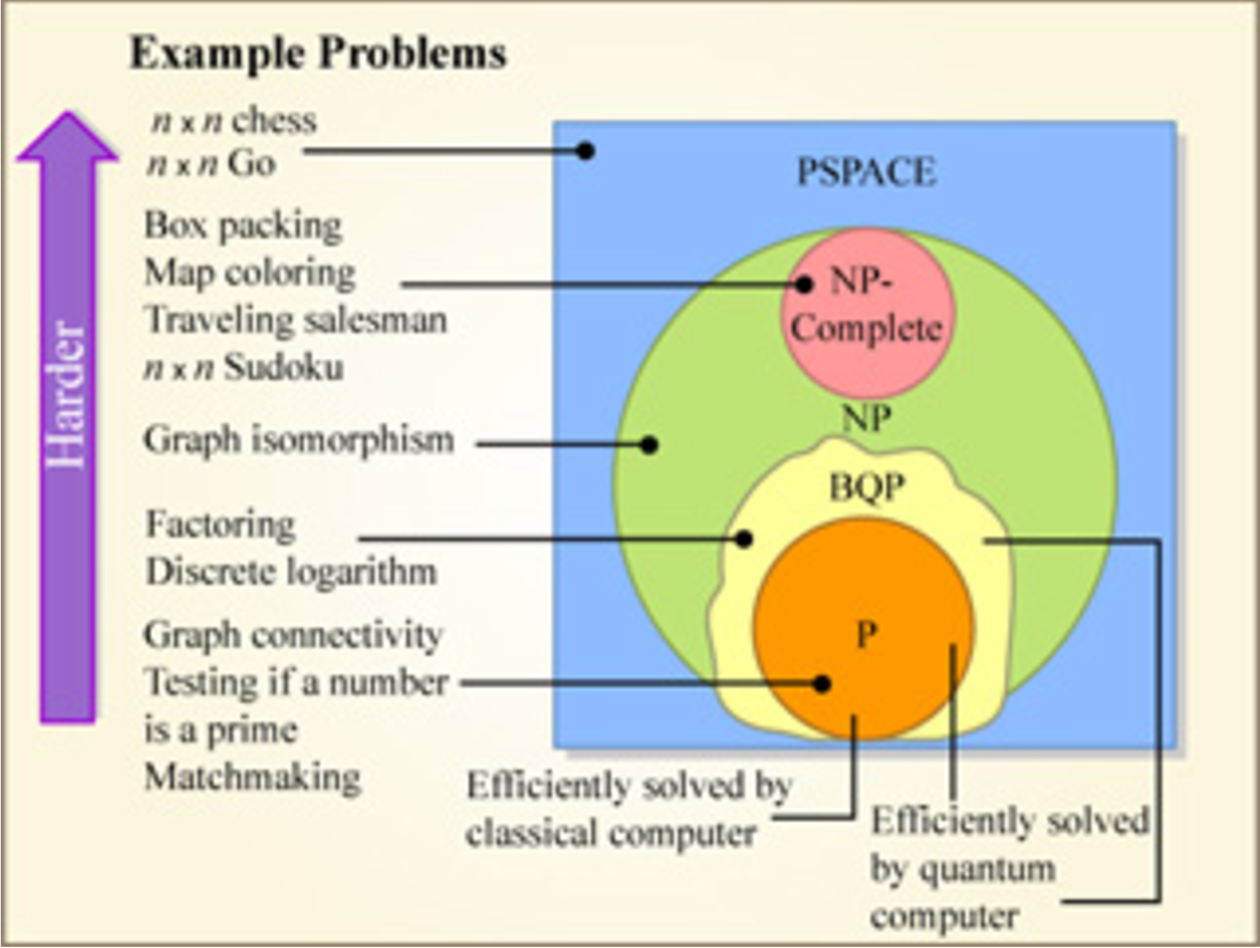
\includegraphics[width=\textwidth]{ai_complexity}
  \caption{La complejidad de algunos problemas en computación. En particular, el \emph{ajedrez}
    y el \emph{go} han sido dos juegos de mesa de gran interés en inteligencia artificial. La historia
    relata que en 1997 la computadora \emph{Deep Blue} de IBM fue capaz de vencer al gran campeón Garry Kaspárov.
    No obstante, su requerimiento de guardar una cantidad \emph{polinomial} de memoria, hacen que en la
    actualidad se estudien modelos capaces de aprender a jugar tanto ajedrez como go, a partir de la observación de partidas.
    (Tomado de (\url{https://ocw.mit.edu/courses/electrical-engineering-and-computer-science/6-845-quantum-complexity-theory-fall-2010/}))}
\end{figure}


El \textbf{aprendizaje automático} (\emph{machine learning} en inglés) es la rama de la IA que trata con algoritmos que son capaces\
de tratar con información estructuralmente incierta (o ruidosa) y generar modelos internos para\
la toma de decisiones. Un agente equipado con la habilidad de aprender automáticamente\
se beneficia de grandes cantidades de ejemplos de un problema, pues su objetivo ahora es\
llegar al mejor modelo, estadísticamente hablando.

\subsection{Las diferentes formas con las que una máquina aprende}

\noindent
La mayoría de los retos computacionales tienen como solución un programa determinístico. Su objetivo\
radica en que dada una entrada $\vec{x}$, el programador diseña en su mente un algoritmo $h$ que calcule\
la salida deseada $z = h(\vec{x})$.\par
En cambio para estimar $z$, en aprendizaje automático, el programador o científico de datos propone un \emph{modelo} $h$\
que sea \emph{entrenado} con respecto a una función objetivo (o de error) $J$, optimizando así, una posible\
solución $\hat{z}$. Todo esto se hace teniendo en cuenta un conjunto de \emph{parámetros} del modelo y\
un conjunto de datos muestrales $\mathcal{D}$.

\begin{figure}[h]
  \centering
  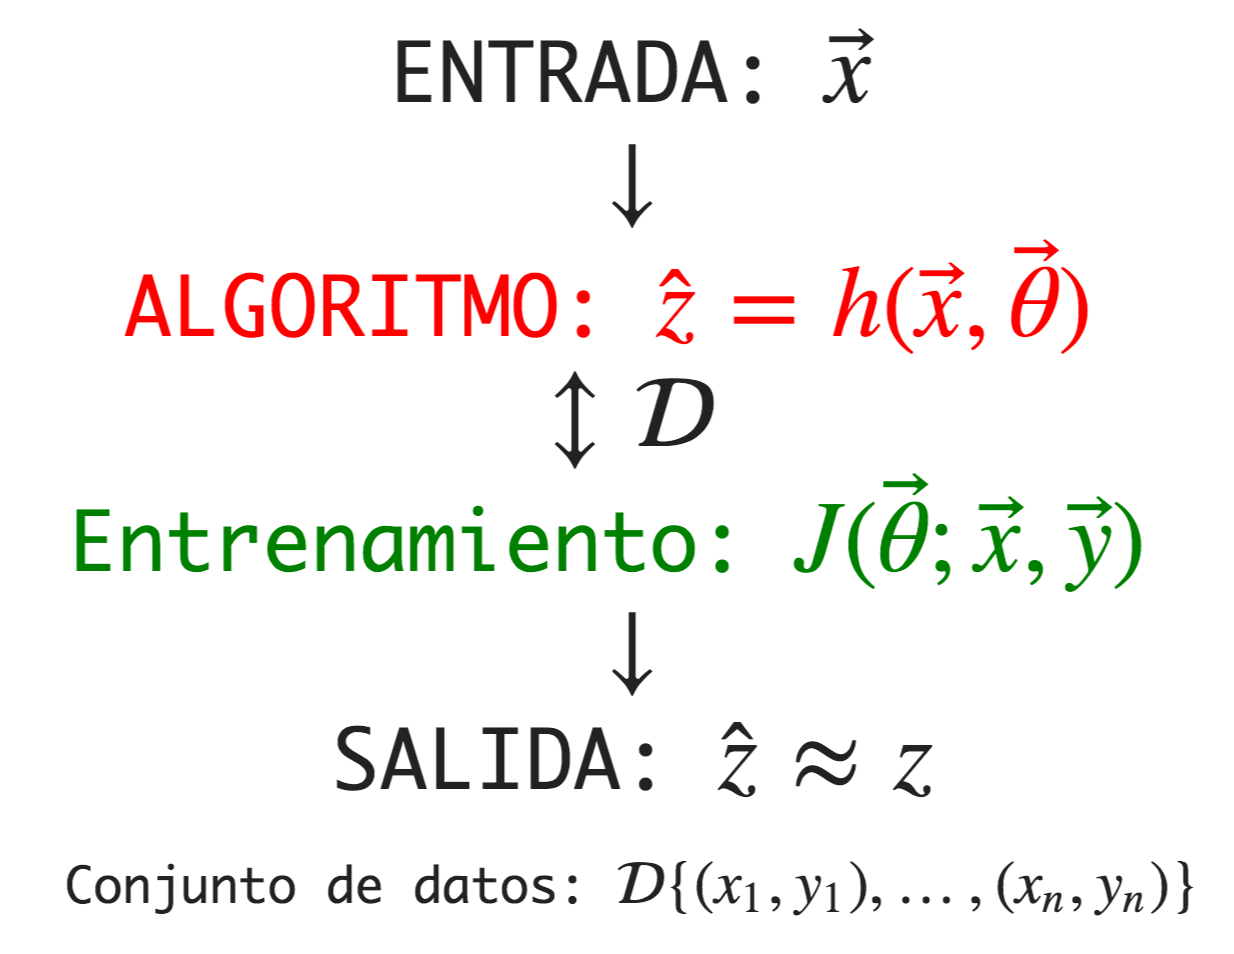
\includegraphics[width=\textwidth]{ml}
  \caption{Las tres fases del aprendizaje automático supervisado.
    (Elaboración propia.)}
\end{figure}

Las maneras de hacer aprendizaje automático dependen de cómo está constituido el conjunto de datos con el\
que se trabaja. En \textbf{aprendizaje supervisado}, se modelan fenómenos a través de muchos ejemplos\
\emph{etiquetados}, es decir, el conjunto de datos puede ser visto como
\begin{equation}
  \mathcal{D} = \{(x_1, y_1),\ldots,(x_n, y_n)\}.
\end{equation}
En este caso, se dice que $\mathcal{D}$ contiene $n$ ejemplos etiquetados: a $\vec{x}$ y a $\vec{y}$ se\
les puede ver como instancias de posibles entradas y salidas del problema $z$, respectivamente. Normalmente,\
$\vec{x}$ se compone de valores numéricos que que fungen como \emph{características} distintivas de la entrada.
El vector $\vec{y}$ puede contener valores de un conjunto discreto (categorías) o continuo.\par
Formalmente, suponiendo que $x_i \in \mathbf{X}$ e $y_i \in \mathbf{Y}$ un algoritmo $h$\
de aprendizaje automático tiene la forma
\begin{equation}
  h: \mathbf{X} \longrightarrow \mathbf{Y}.
\end{equation}
Si $\mathbf{Y}$ es un conjunto finito, entonces decimos que el problema es de \textbf{clasificación}, mientras\
que si es infinito (y denso) es de \textbf{regresión}.\par
En la presente tesis, se trabajará únicamente con aprendizaje supervisado, pues cada uno de los memes de\
muestra ($\mathbf{X}$), está etiquetado con una o varias leyendas ($Y$). El reto consiste en construir un\
modelo que sea capaz de capturar las características más importantes de la imagen y que las asocie a un\
\emph{modelo de lenguaje}. Todo esto será profundizado más adelante.\par
Para terminar con la teoría general de aprendizaje automático, vale la pena destacar que es posible\
realizar \textbf{aprendizaje no supervisado}. Esto se logra mediante un conjunto de datos que carece\
de salidas $\mathbf{Y}$; el objetivo de un agente será desvelar los patrones que comparten las características\
dadas, es decir, aprender a agrupar los datos mediante el uso de similitudes estadísticas.\
\textbf{Aprendizaje por refuerzo} es otra manera de hacer aprendizaje automático y se basa en\
un entrenamiento en el que el ajente debe de maximizar un puntaje debido a una retroalimentación\
dada por sus acciones. Esto último va más allá de los objetivos de esta tesis.
